\chapter{Probléma definíció}
Számos esettanulmány és irodalmi példa esetében a batch méretek nem rögzítettek, és ha több egység képes elvégezni egy részfeladatot, akkor párhuzamosan tehetik meg azt. Ez a fajta probléma meghatározás különösen gyakran az throughput vagy bevétel maximalizációs probléma esetén jelentkezik, de megjelenhet a makespan minimalizálásnál is. Az idő diszkréción alapuló megközelítések meg tudják oldani ezt a problémát, azonban az S-gráf keretrendszer esetén néhány módosítás szükséges.
Az ~\ref{throughput_alg} ábrán látható algoritmus megköveteli, hogy a recept rögzített legyen, valamint egy termékhez tartozó batch jövedelme is előre ismert legyen. Az előbb említett problémák esetén viszont egyik sem garantált. 
A javasolt megközelítés szemléltetésére a Kondili és munkatársaitól \cite{kondili} származó példát veszem igénybe. Ez látható \ref{kondiliPelda} ábrán.

A folyamat 5 taszkból áll: fűtésből, 3 darab reakcióból, és az elválasztásból. Ezekhez 4 berendezés áll rendelkezésre, a fűtőtest és szeparátor, mindkettő 100 kilogrammos kapacitással a fűtés és elválasztás folyamatához. A három reakciós folyamathoz van 2 darab reaktor ugyanakkor feldolgozása idővel. A kapacitásuk eltér, egyiké 80 kilogramm a másiké pedig 50 kilogramm, de lehet őket párhuzamos igénybe venni. Feltételezzük, hogy az összes egység képes a kapacitásuknál kisebb terheléssel működni, azaz nincs teherbírásuknak alsó határa. A folyamat során két termék készül azonos profittal. A következő korlátozások fennállnak: nem marad semmilyen köztes anyag a termelő folyamat végén, nem lehet csak az egyes számú terméket gyártani, illetve nincs tárolásra lehetőség a folyamat során.
\begin{figure}[H]
\begin{center}
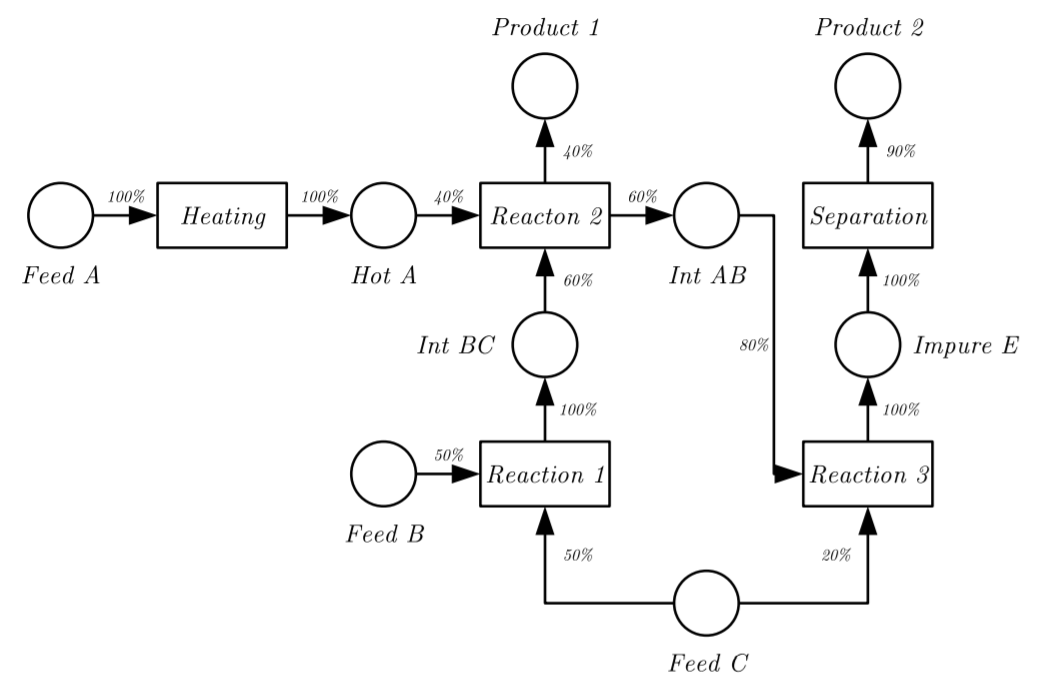
\includegraphics[scale=0.65]{kondiliPelda}
\caption{Kondili példafeladata}
\label{kondiliPelda}
\end{center}
\end{figure}
Mindegyik reakciós folyamat elvégezhető egyik vagy másik reaktor által, illetve ezekkel párhuzamosan. Ez $3^3 = 27$ fix receptet eredményez, amelyek különböző batch méret intervallummal rendelkezhetnek. Mindegyik esetben különálló S-gráf receptet kell létrehozni, hogy a korábban említett S-gráf algoritmust igénybe lehessen venni profit maximalizálásra, így a keresési terület 27 dimenziós térré válna. Ez óriási CPU igényhez vezetne az optimalizálás során, ezért az esetek számának csökkentése elengedhetetlen.

$$Tablazatot ide $$

Ha megnézzük a táblázatot észrevehető, hogy csupán néhány érték ismétlődik. Ennek oka az anyagok egyensúlyából származik. Például, hogy ha mind az R1-et mind az R2-t hozzárendeljük a hármas számú reakcióhoz ahelyett, hogy csak az R1 lenne hozzárendelve, akkor sem lesz nagyobb a kimenet, mert a korábbi reakciókból származó pótlás nem éri el a szükséges szintet. Ha a két különböző eset, $c$ és $c'$, ugyanakkora maximális jövedelemmel rendelkezik, de a $c$ eset csak kisebb részét használja a $c'$ által használt egységeknek. Ekkor az mondjuk, hogy a $c$ \textit{dominálja} a $c'$-t. A példából látható, hogy a 9-es eset dominálja a 27-es esetet. Továbbá a 24-es eset dominálva van a 4,5,6,13,14,15,22,23 esetek által. Megállapíthatjuk, hogy ha egy eset legalább egy másik által dominálva van, akkor azt kizárhatjuk a vizsgálatból, mert az továbbra is garantálva van, hogy megtalálja az optimális megoldást. A következő táblázat tartalmazza azokat az eseteket, amelyek nincsenek dominálva más esetek által. 	

$$Tablazatot ide $$

Ezután a esetszám csökkenés után is még mindig 11 esetet kellene az S-gráf algoritmusnak megvizsgálni. Annak érdekében, hogy tovább csökkenjen ez a szám több esetet is össze lehet vonni. Például a 4-es és 5-ös eset teljes mértékben megegyezik, azzal a kivétellel, hogy a harmadik reakciós folyamatot más reaktor végzi. Ezt a két esetet össze lehet vonni úgy, hogy a harmadik reakciónál R1 vagy R2-es reaktor, $R1 \vee R2$, üzemel. A következő táblázatban látható a végleges összevonás eredménye.

$$Tablazatot ide $$




